\section{Теоритические сведения}
Баллистическим гальванометром называют электроизмерительный прибор магнитоэлектрической системы, отличающийся высокой чувствительностью к току и сравнительно большим периодом колебаний подвижной системы (рамки).

Главной частью баллистического гальванометра является подвешенная на вертикальной
нити рамка, помещённая в поле постоянного
магнита. Вырез цилиндрической формы в полюсах магнита и ферромагнитный цилиндр на
оси системы делают поле в зазоре радиальным.
Скреплённое с рамкой зеркальце служит для измерения угла поворота рамки. К рамке прикреплён полый цилиндр, который сильно увеличивает момент инерции и,
следовательно, период колебаний подвижной системы, не очень её утяжеляя. Магнит и подвижная система заключены в защитный кожух. В баллистических гальванометрах применяют сильные постоянные магниты и рамки с большим количеством
витков, подвешенные на тонких нитях с малой упругостью.

\begin{figure}[ht!]
    \center{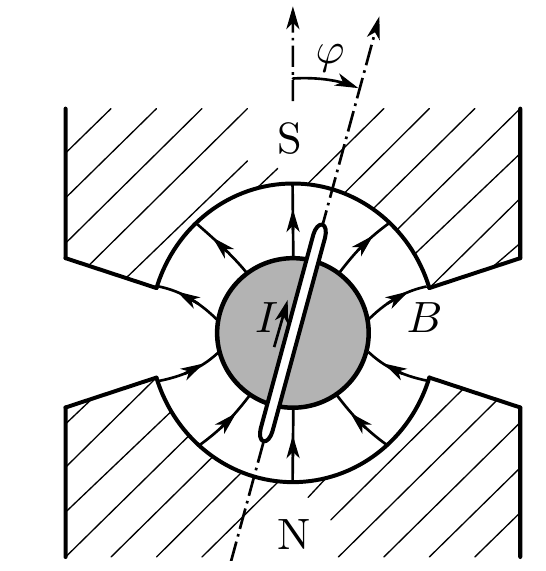
\includegraphics[width=0.5\linewidth]{../img/th1.png}}
\end{figure}

Баллистический гальванометр позволяет измерять как постоянный
ток (стационарный режим), так и заряд, протекший через рамку за
некоторое время (баллистический режим). В баллистическом режиме
гальванометр может работать, если время протекания заряда много
меньше периода собственных колебаний подвижной рамки. Поэтому период колебаний рамки делают большим (10 секунд). Это время учитывает реакцию экспериментатора, которому надо успеть сделать отсчёт максимального отклонения рамки.

\subsection{Уравнение движения рамки в магнитном поле}
На помещённую в магнитное поле рамку гальванометра, по которой
течёт ток, действуют момент сил закрученной нити, момент сил трения
(сопротивление воздуха и т. п.) и момент магнитных сил (сил Ампера).
Последний можно условно разделить на две составляющие: момент, действующий на составляющую тока, обусловленную ЭДС внешней цепи,
и тормозящий момент, возникающий благодаря электромагнитной индукции (электромагнитное торможение). Рассмотрим каждый из этих
моментов в отдельности.

Механический момент $M_{1}$ упругих сил нити пропорционален углу поворота рамки:
\[
    M_{1} = -D \varphi
\]
$D$~--- модуль кручения нити, $ \varphi$~--- угол поворота рамки от положения равновесия.

Момент сил вязкого трения пропорционален угловой скорости рамки:
\[
    M_{2} = - \beta \dot{ \varphi}
\]
Пусть прямоугольная рамка с числом витков $N$,  обтекаемая по контуру током $I_{ \Sigma}$,
помещена в магнитное поле с постоянной индукцией $B$. Тогда на каждую боковую сторону
рамки действуют силы, равные $F_{A} = lNBI_{ \Sigma}$.
\[
    M_{3} = BSNI_{ \Sigma} = 2rlBNI_{ \Sigma}
\]

В рамке, движущейся в магнитном поле с угловой скоростью $\dot{ \varphi}$, наводится ЭДС индукции:
\[
    \mathcal{E}_{\text{инд}} = -BSN\dot{\varphi}
\]
\[
    I_{\text{инд}} = \frac{\mathcal{E}_{\text{инд}}}{R_{ \Sigma}}
\]
\[
    R_{ \Sigma} = R_{0} + R
\]
Связанный с ЭДС индукции момент:
\[
   M_{3}^{\text{инд}} = BSNI_{\text{инд}} = -\frac{(BSN)^{2}}{R_{ \Sigma}}\varphi^{2}       
\]
Видно, что этот момент всегда тормозит вращение рамки (электромагнитное торможение).
Причём обычно электромагнитный тормозящий момент значительно превосходит момент сил трения рамки:
$(BSN)^{2}/R_{ \Sigma}\gg \beta_{\text{тр}}$,  поэтому далее мы для простоты расчёта пренебрежём величиной $M_{2}$.

Полный ток через рамку определяется уравнением цепи рамки.
Пусть эта цепь подключена к некоторому внешнему источнику ЭДС.  Тогда, в пренебрежении самоиндукцией рамки и контура, имеем
\[
    I_{\Sigma} = \frac{\mathcal{E} + \mathcal{E}_{\text{инд}}{R_{\Sigma}}} = I + I_{\text{инд}}
\]

$I$~--- составляющая тока, вызванная внешней ЭДС, к которой подключён гальванометр.

Вращение рамки описывается уравнением моментов.
\[
    \ddot{\varphi} + 2\gamma\dot{\varphi} + \omega_{0}^{2} \varphi = KI
\]
\[
    K = BNS/J,\;\;\;2\gamma = \beta + \frac{(BNS)^{2}}{JR_{\Sigma}}\approx\frac{(BNS)^{2}}{JR_{\Sigma}}\,\;\;\;\omega_{0}^{2} = D/J
\]

\subsection{Режим измерения постоянного тока}
Если через рамку пропускать постоянный ток, то, как нетрудно видеть, заменой переменой
уравнение приводится к однородному уравнению вида, описывающему свободные
затухающие колебания. Если подождать достаточно долго, чтобы собственные колебания затухли, в уравнении можно положить $\dot{ \varphi} = 0$, $\ddot{\varphi} = 0$,  так что угол поворота рамки определится формулами
\[
    \varphi = KI/\omega_{0}^{2} = BSNI/D = S_{I}I = I/C_{i}
\]
$S_{I} = \varphi/I = BSN/D$~--- чувствительность, $C_{I} = 1/S_{I}$~--- динамическая постоянная.

\subsection{Свободные колебания рамки}
Исследуем свободное движение рамки, т. е. движение в отсутствие внешних источников, когда $I=0$.
\[
    \ddot{ \varphi} + 2\gamma\dot{ \varphi} + \omega_{0}^{2}\varphi = 0
\]

\begin{enumerate}
    \item $ \gamma < \omega_{0}$ (колебательный режим).
    Движение колебательной, период равен
    \[
        T_{1} = 2\pi/\sqrt{\frac{D}{J}-\frac{(BSN)^{4}}{(2JR_{\Sigma})^{2}}}
    \]
\item $ \gamma = \omega_{0}$ (критический режим).
    \[
        R_{\text{кр}} = \frac{(BSN)^{2}}{2\sqrt{DJ}} - R_{0}
    \]
\item $ \gamma > \omega_{0}$ (затухание велико — случай переуспокоенного гальванометра).
        
\end{enumerate}
\subsection{Режим измерения заряда}
Как уже было отмечено, период свободных колебаний баллистического гальванометра благодаря искусственному увеличению момента инерции рамки оказывается очень большим (порядка десяти секунд). Если
пропустить через рамку короткий импульс тока, то можно считать, что
весь ток успевает пройти при неотклонённом положении рамки. Рамка, однако, при этом получает толчок, в результате которого возникаетдвижение, описываемое уравнением свободных колебаний.

\[
    \dot{\varphi}(\tau) = Kq
\]

Таким образом, при пропускании короткого импульса тока через баллистический гальванометр начальная угловая скорость движения рамки
пропорциональна полному электрическому заряду, прошедшему через рамку за всё время импульса.
Легко увидеть, что наибольший угол $\varphi_{max}$,  на который отклоняется рамка, также пропорционален $q$.

Величина $C_{q} = q/\varphi_{max}$ называется баллистической постоянной гальванометра. Баллистическая постоянная наряду с динамической является важнейшей характеристикой гальванометра, но в отличие от динамической она существенно зависит от режима работы гальванометра (от сопротивления цепи). Величина
$S_{q} = 1/C_{q}$ = называется чувствительностью гальванометра к заряду.

Выбирая оптимальный режим работы, приходится одновременно исходить из двух противоречивых требований: желания получить максимальную чувствительность гальванометра к заряду и стремления по возможности сократить время, затрачиваемое на измерения. Расчёт показывает, что максимальный отброс достигается при полном отсутствии
затухания (тормозящий индукционный ток отсутствует при обрыве вцепи):
\[
    \varphi_{max}^{\text{св}} = \frac{Kq}{\omega_{0}}
\]
В этом случае, однако, возникшие в результате отброса колебания рамки
не будут успокаиваться, и прибор не скоро сможет быть использован для
повторных измерений. Поэтому обычно заботятся о том, чтобы затухание гальванометра не было слишком малым. Кроме того, отметим, что
затухание приводит к тому, что зайчик начинает вести себя более спокойно и слабее реагирует на посторонние электрические и механические импульсы.

Как правило, удобнее всего работать в режиме, близком к критическому. При этом обеспечивается и быстрое затухание колебаний, и чувствительность прибора достаточно велика.
\[
    \varphi_{max}^{\text{кр}} = \frac{Kq}{\omega_{0}e}
\]
Таким образом, в критическом режиме максимальное отклонение зайчика в $e$ раз меньше, чем в режиме свободных колебаний. Отсюда, в частности, следуют соотношения между баллистическими постоянными
и чувствительностями гальванометра, работающего в режиме свободных
колебаний и в критическом режиме:
\[
    \frac{C_{q}^{\text{кр}}}{C_{q}^{\text{св}}} = e
\]

